%****************************************************
%	CHAPTER 4 - DATA COLLECTION
%****************************************************
\chapter{Data Collection}
\label{ch:data_collection}
%====================================================

%====================================================
\section{Data Collection Apparatus}
\label{sec:ch4.section1}
%----------------------------------------------------

All \ac{LiDAR} data collected for this investigation used one of two apparatus. For the data collected from the Aalto University Ice and Wave Tank, the Livox Avia and a laptop running Windows 11 and the Livox SDK were used. For every other dataset, The Livox Avia and a laptop running Ubuntu 20.04 and \ac{ROS} Noetic were used.

In each case, the Avia's non-repetitive scanning pattern was used for data capture as it provides a wider \ac{FOV} than the non-repetitive scanning pattern and captures more unique data points. The sensor was configured to operate exclusively in single return mode, as the target environment is not expected to produce useful multiple returns. Data was captured at the sensor's default rate of 10 Hz for the point cloud frames and 200 Hz for the \ac{IMU} data.

%====================================================
\section{Characterisation and Experimental Data Collection}
\label{sec:ch4.section2}
%----------------------------------------------------

The following sections detail experiments conducted to characterise the Livox Avia sensor's behaviours under controlled conditions that simulate some conditions expected during in-situ data collection.

The first experiment detailed in Section \ref{subsec:ch4.section2.subsec1} investigates the sensor's ability to resolve known geometric shapes at known distances and angles, from a stationary platform. 

The second experiment detailed in Section \ref{subsec:ch4.section2.subsec2} was conducted to collect data from the Avia's \ac{IMU} while the sensor was subjected to known motion. This data was used to investigate the feasibility of compensating for the motion of a moving observation platform.

%----------------------------------------------------
\subsection{Stationary Characterisation Experiment}
\label{subsec:ch4.section2.subsec1}

To simulate conditions similar to those that may be experienced when observing the ocean surface from a research vessel, such as the \textit{S.A. Agulhas II}, a field experiment was conducted using the Livox Avia. The experiment took place on the University of Cape Town's rugby field, using two large sheets of hardboard as target surfaces.

The Avia was mounted on a tripod and placed on a terrace above the rugby field at a height of 9.1 metres above the ground, angled downwards at an angle of 16° from the horizontal, as seen in Figure \ref{fig:field_setup}. These dimensions and angles were selected to simulate the expected observation geometry when mounted on a research vessel, as informed by the data collection setup detailed in Section \ref{subsec:ch4.section3.subsec2}.

%----------------------------------------------------
\begin{figure}[H]
\centering
\begin{minipage}{.5\textwidth}
  \centering
  \includegraphics[width=0.95\linewidth]{figs/field_setup.png}
  \caption{\textbf{Data collection Apparatus}}
  \label{fig:field_setup}
\end{minipage}%
\begin{minipage}{.5\textwidth}
  \centering
  
\includegraphics[width=0.95\linewidth]{figs/edited_level.png}
  \caption{\textbf{Avia Angle of Depression.}}
  \label{fig:angle}
\end{minipage}
\end{figure}
%----------------------------------------------------

Two sheets of hardboard, 1220 x 1220 mm each, a similar in size to a small pancake ice floe, were used to create the target surfaces. The boards were deformed using string to create concave and convex shapes, 1220 mm in length, 1130 mm in width, with a maximum height of 180 mm, as shown in Figure \ref{fig:boards}. The concave and convex shapes were chosen to investigate the sensor's ability to resolve simple curved surfaces and ensure that some amount of shadowing would occur in the point cloud data. Four variations (Targets A, B, C and D) of the target boards were created by orienting the axis of curvature both parallel and perpendicular to the sensor's line of sight. Targets A and B had the axis of curvature perpendicular to the sensor's line of sight, see Figure \ref{fig:boards}, while Targets C and D had the axis of curvature parallel to the sensor's line of sight, see Figures \ref{fig:target_c} and \ref{fig:target_d}. The boards were placed on the rugby field at a distance of approximately 40 metres from the Avia, near to the centre of the sensor's \ac{FOV} to ensure a high point density on the target surfaces.

%----------------------------------------------------
\begin{figure}[H]
    \centering
    
\includegraphics[width=0.95\textwidth]{figs/field_boards.JPG}
    \caption{\textbf{Target Boards.} Target A on the left, target B on the right.}
    \label{fig:boards}
\end{figure}
%----------------------------------------------------

%----------------------------------------------------
\begin{figure}[H]
\centering
\begin{minipage}{.5\textwidth}
  \centering
  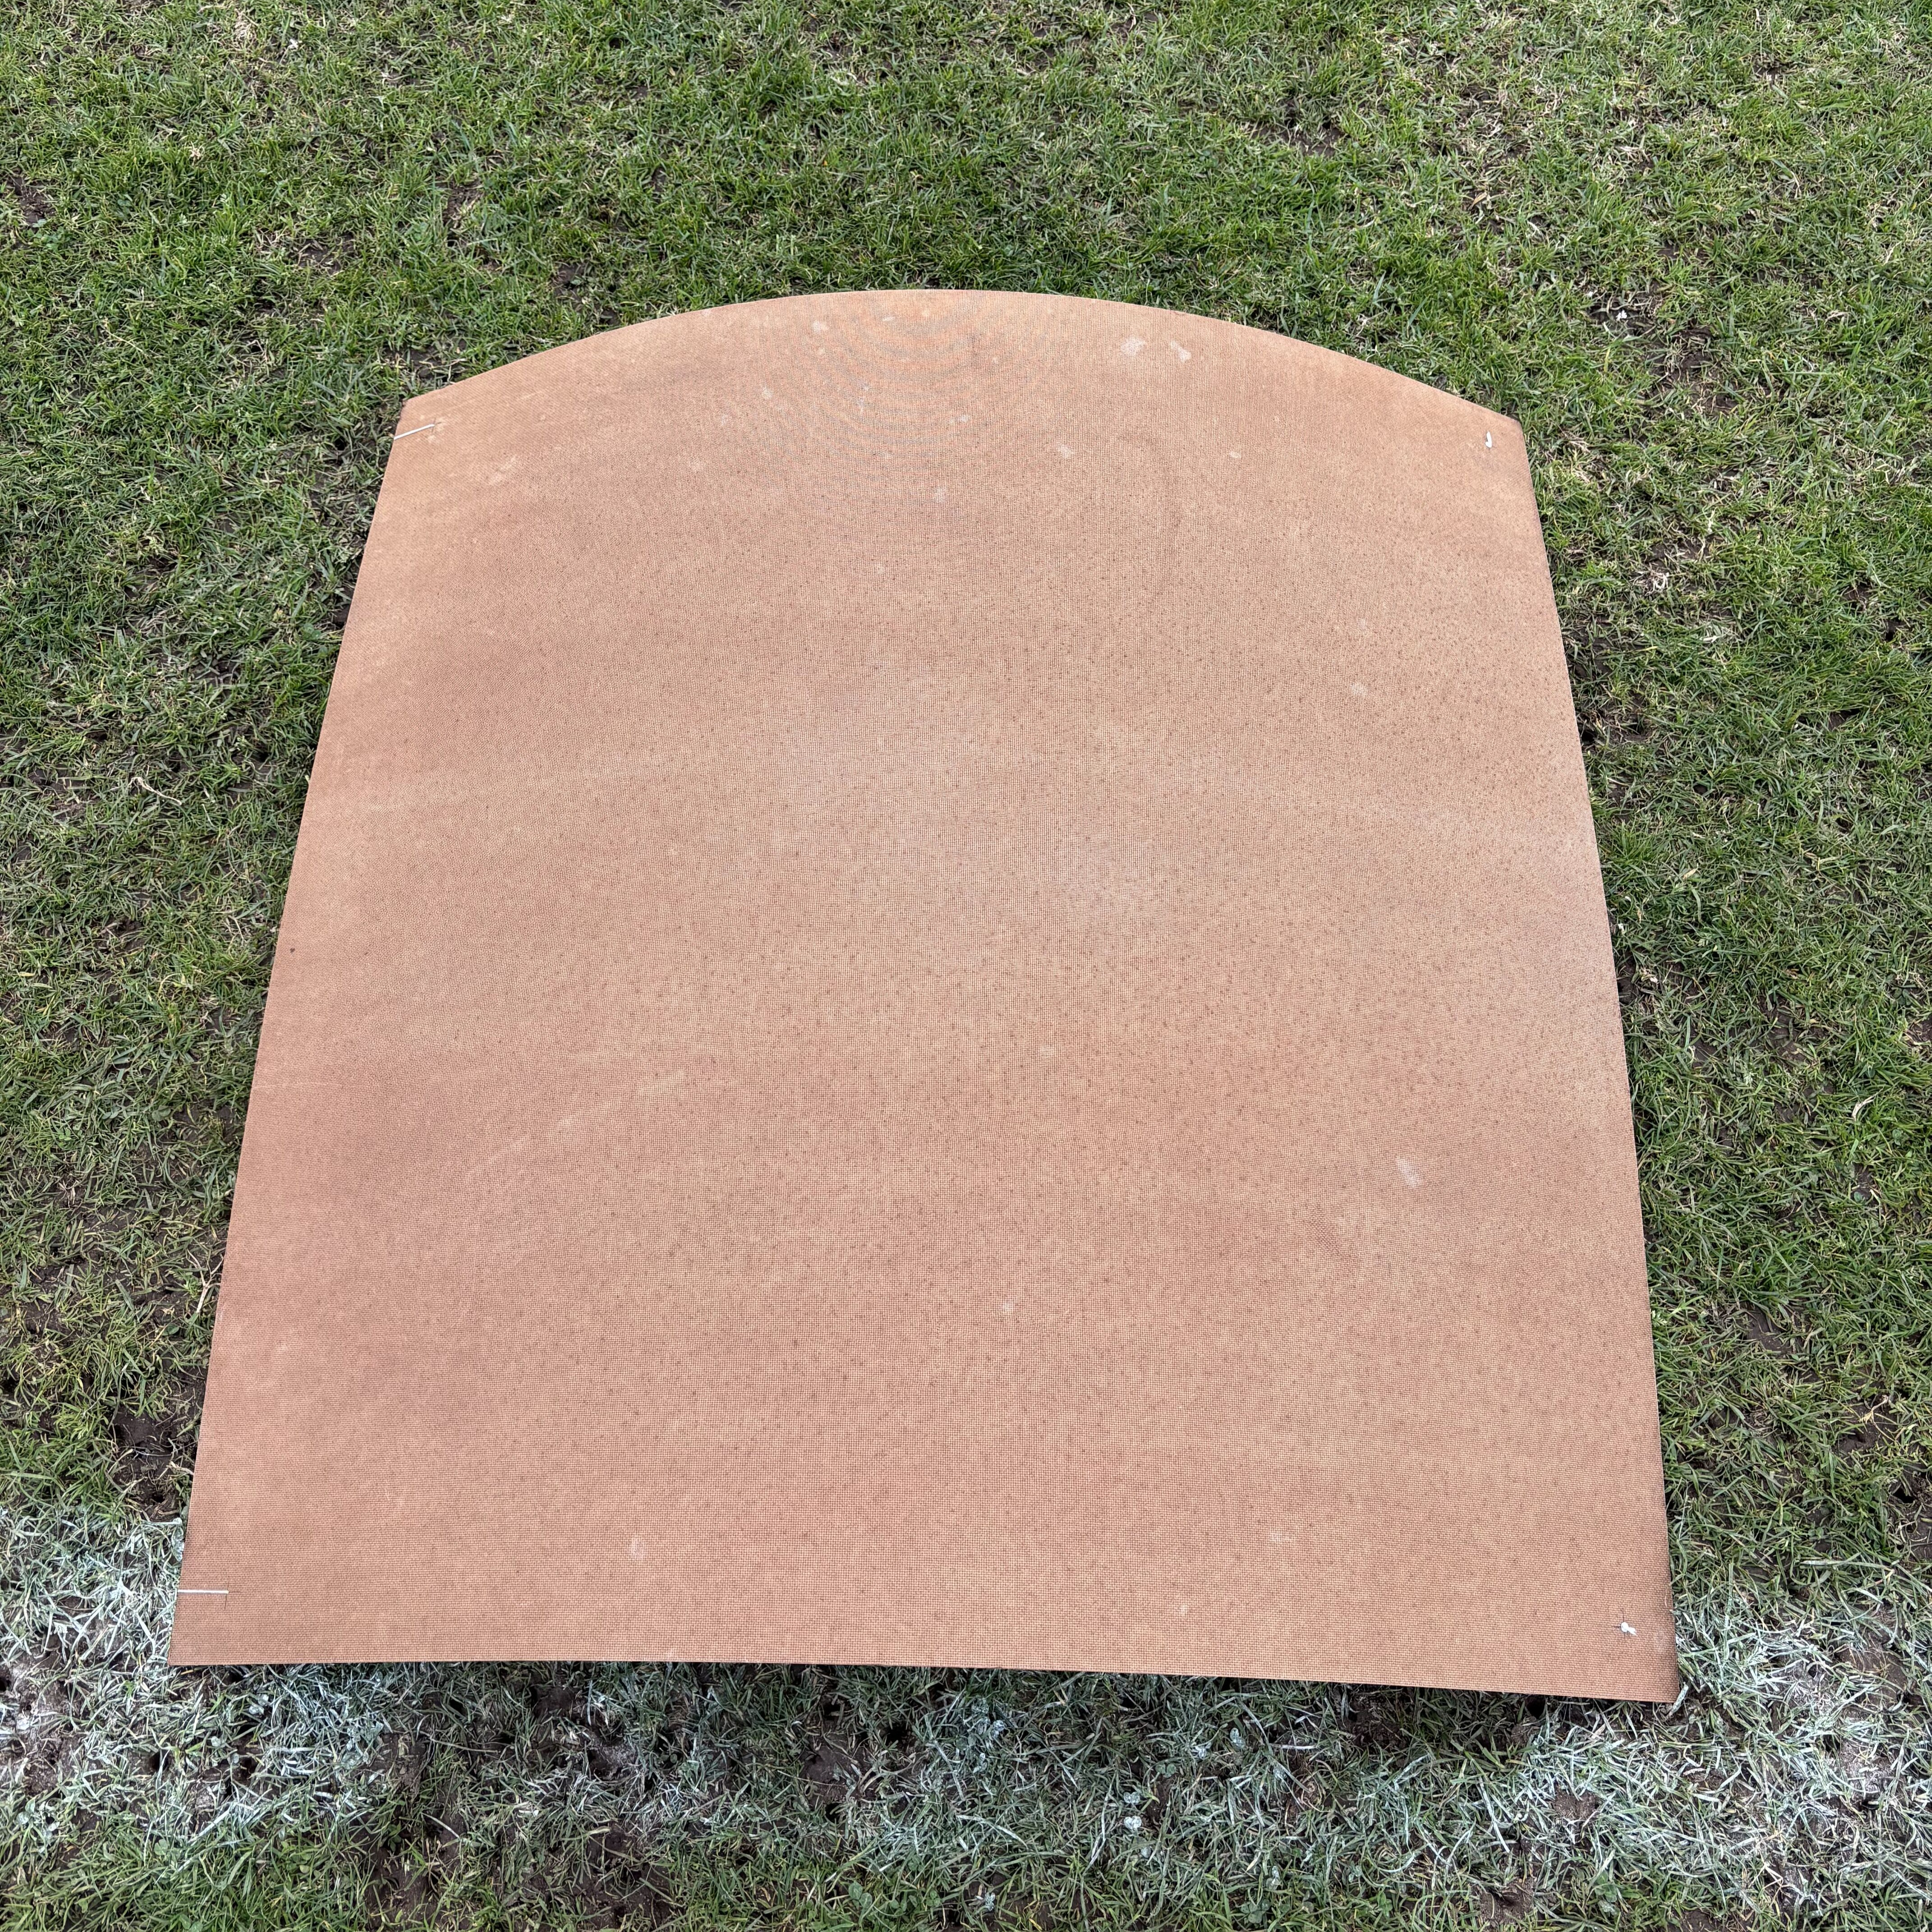
\includegraphics[width=0.95\linewidth]{figs/board_c.jpg}
  \caption{\textbf{Target C.}}
  \label{fig:target_c}
\end{minipage}%
\begin{minipage}{.5\textwidth}
  \centering
  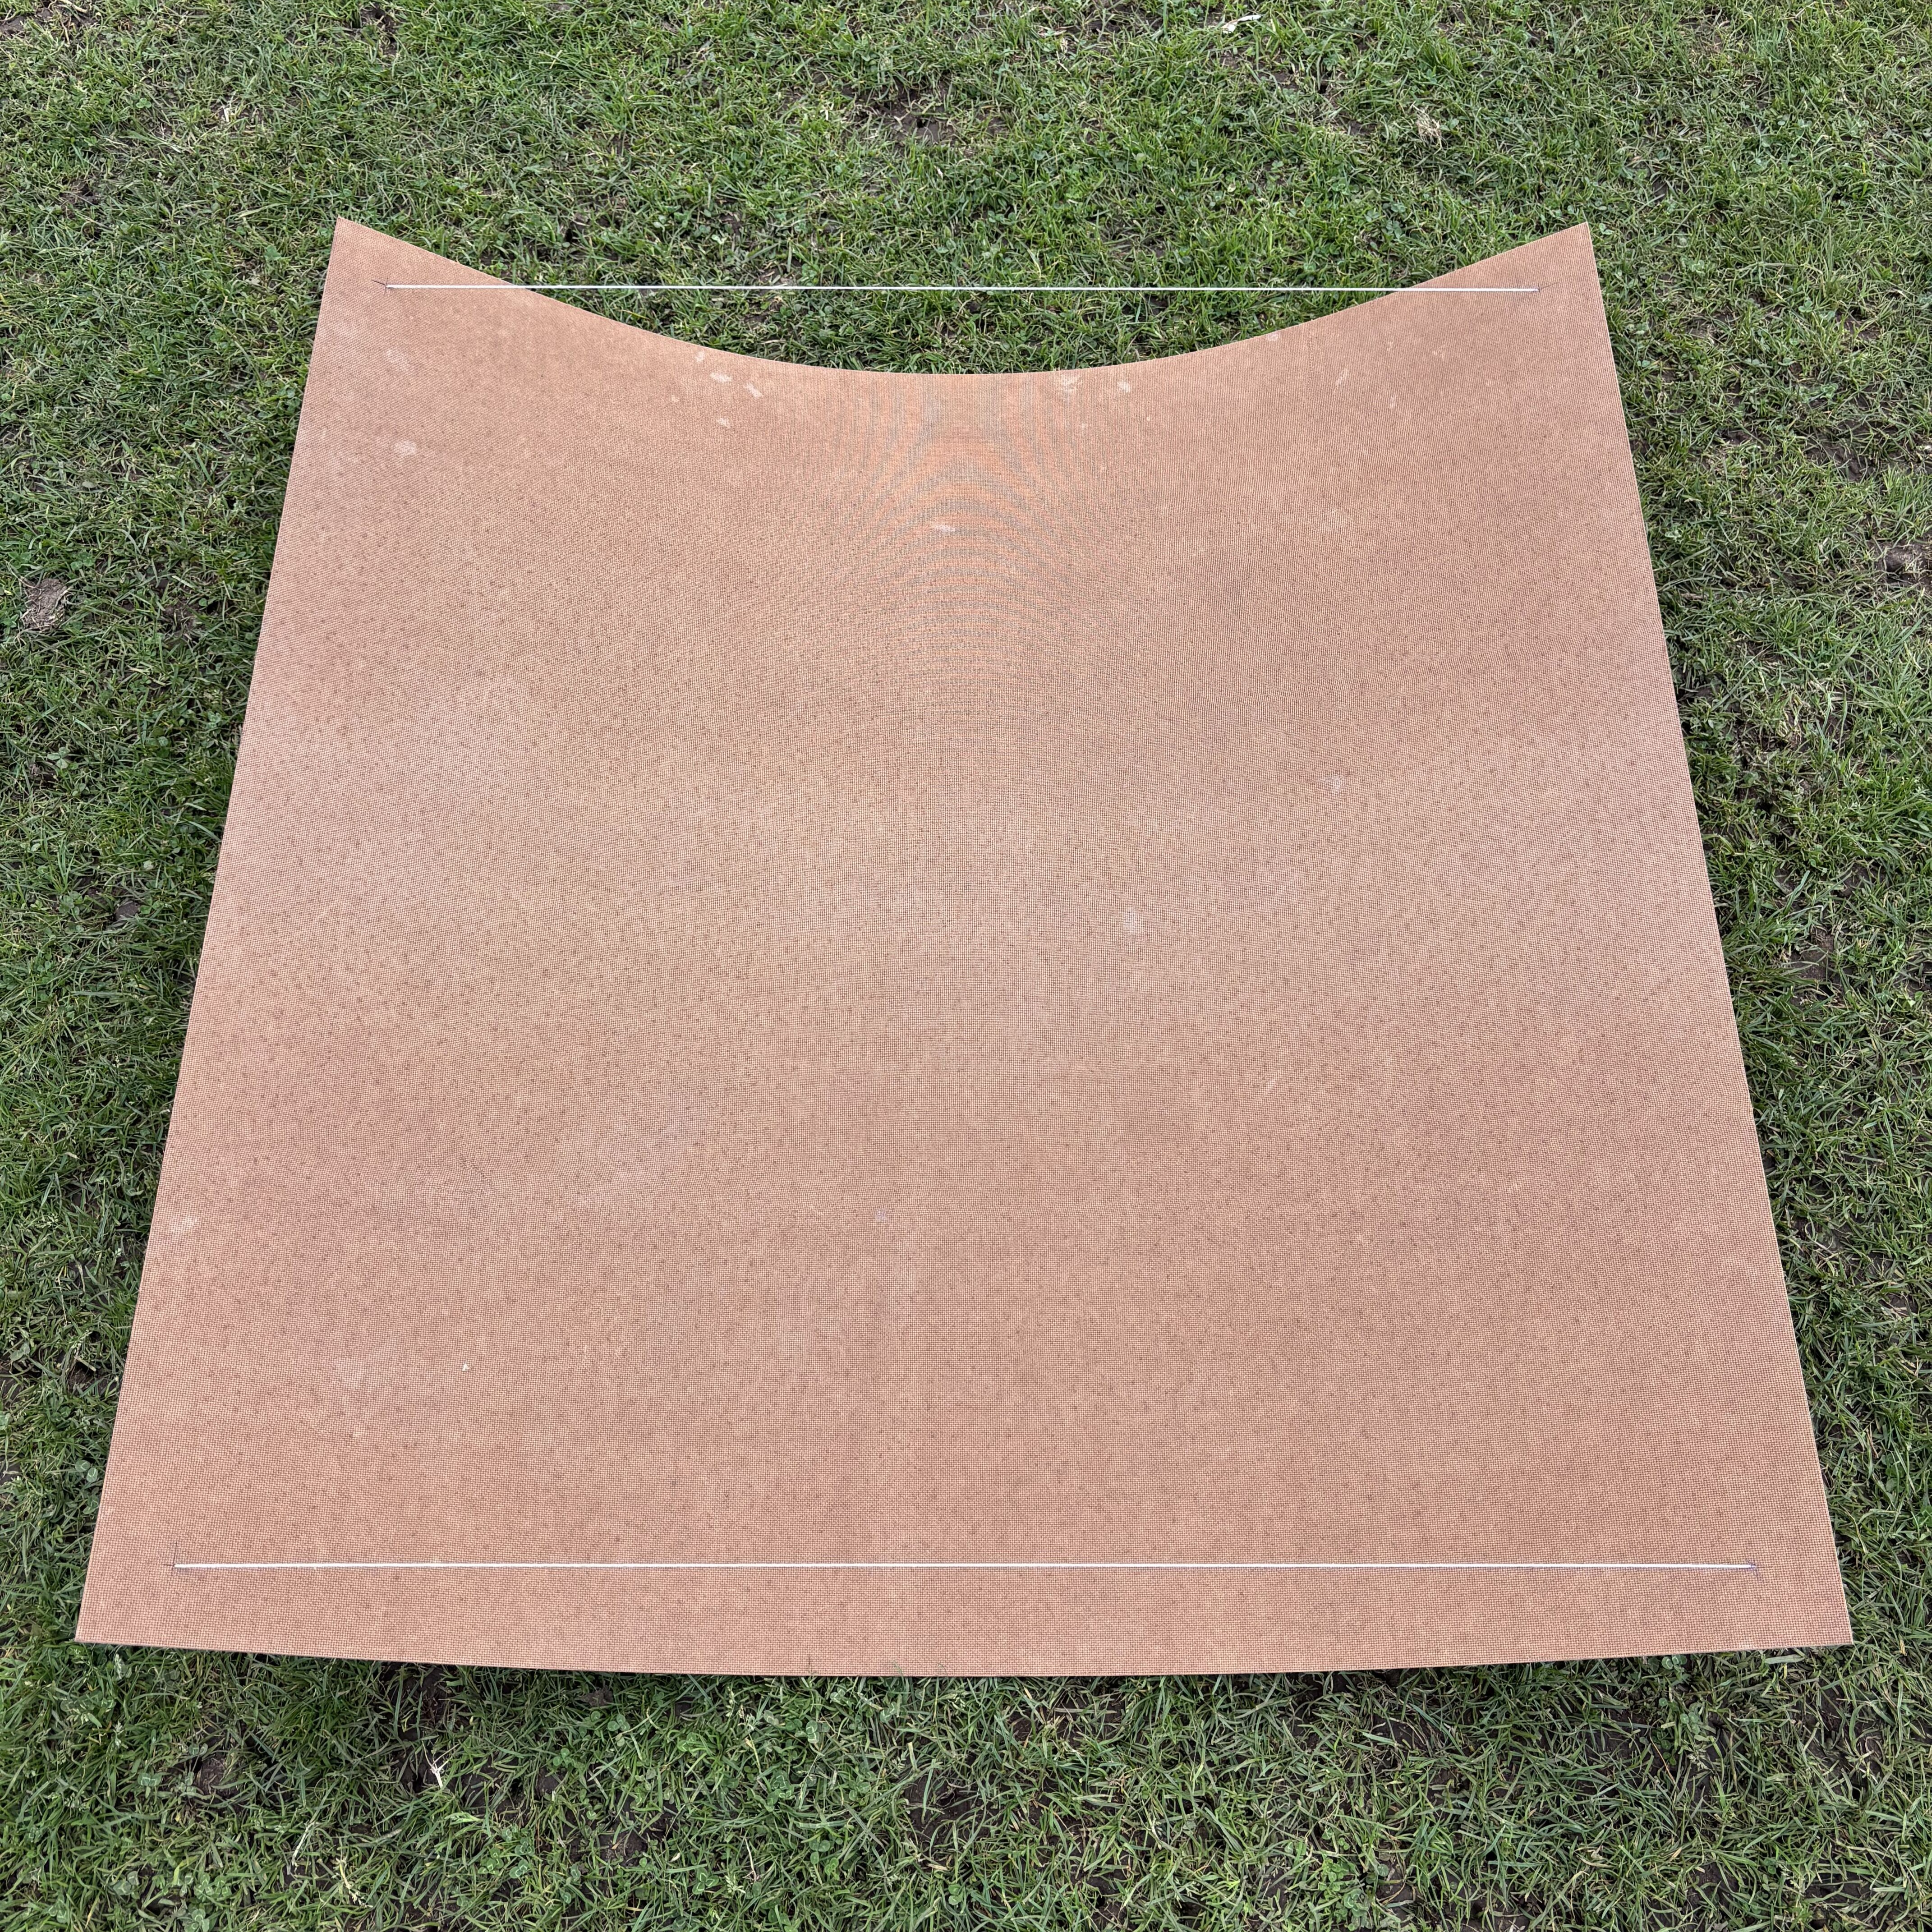
\includegraphics[width=0.95\linewidth]{figs/board_d.jpg}
  \caption{\textbf{Target D.}}
  \label{fig:target_d}
\end{minipage}
\end{figure}
%----------------------------------------------------

The Avia collected a minimum of 75 point cloud frames of each target.

%----------------------------------------------------
\subsection{Simulated Motion Experiment}
\label{subsec:ch4.section2.subsec2}

To investigate the feasibility of using the Avia's \ac{IMU} data to compensate for the motion of a moving observation platform, an experiment was conducted to collect \ac{IMU} data from the Avia while it was subjected to known motion.

To apply known motion to the Avia, a Stewart platform was used to manipulate the sensor. A Stewart platform is a device that has the ability to manipulate its target platform in 6 degrees, namely linear translations along its X, Y and Z axes and rotation around its the X, Y, and Z axes (\cite{stewartPlatformSixDegrees1965}). The Stewart platform used for this experiment was designed and built a former student from the University of Cape Town (\cite{clarkStewart2018}). The platform had been used sporadically since its construction in 2018, and had undergone many repairs and part replacements, resulting in irregular performance that did not meet the original design specifications. To overcome this limitation, a motion capture system was employed to record ground-truth motion data for comparison and validation.

The motion capture system used in this experiment was manufactured by \href{https://optitrack.com}{OptiTrack}, who provided all sensors, software and supporting equipment. The system consists of 4 OptiTrack PrimeX 13 cameras and 3 OptiTrack PrimeX 13W (wide angle) cameras, all managed by a PC running OptiTrack's Motive software. Both camera types record data at a rate of 240 Hz, with the PrimeX 13 having a listed 3D accuracy of +/- 0.02 mm (\cite{PrimeX13Depth}), and the PrimeX 13W having a listed 3D accuracy of +/- 0.03 mm (\cite{PrimeX13WDepth}). The system makes use of passive infrared reflective markers to track the position of the target over time. The data collected by the motion capture system was not time-synchronised with the Avia's \ac{IMU} data.

As this experiment is intended to be a preliminary investigation into the feasibility of using \ac{IMU} data for motion compensation, only rotational motion, and no translational motion was applied to the Avia. The Avia had six motion capture markers attached to it, (see Figure \ref{fig:markers}) and was mounted to the Stewart platform using a custom 3D-printed mount, as seen in Figure \ref{fig:motion_setup}.

%----------------------------------------------------
\begin{figure}[H]
\centering
  \begin{minipage}{.5\textwidth}
    \centering
    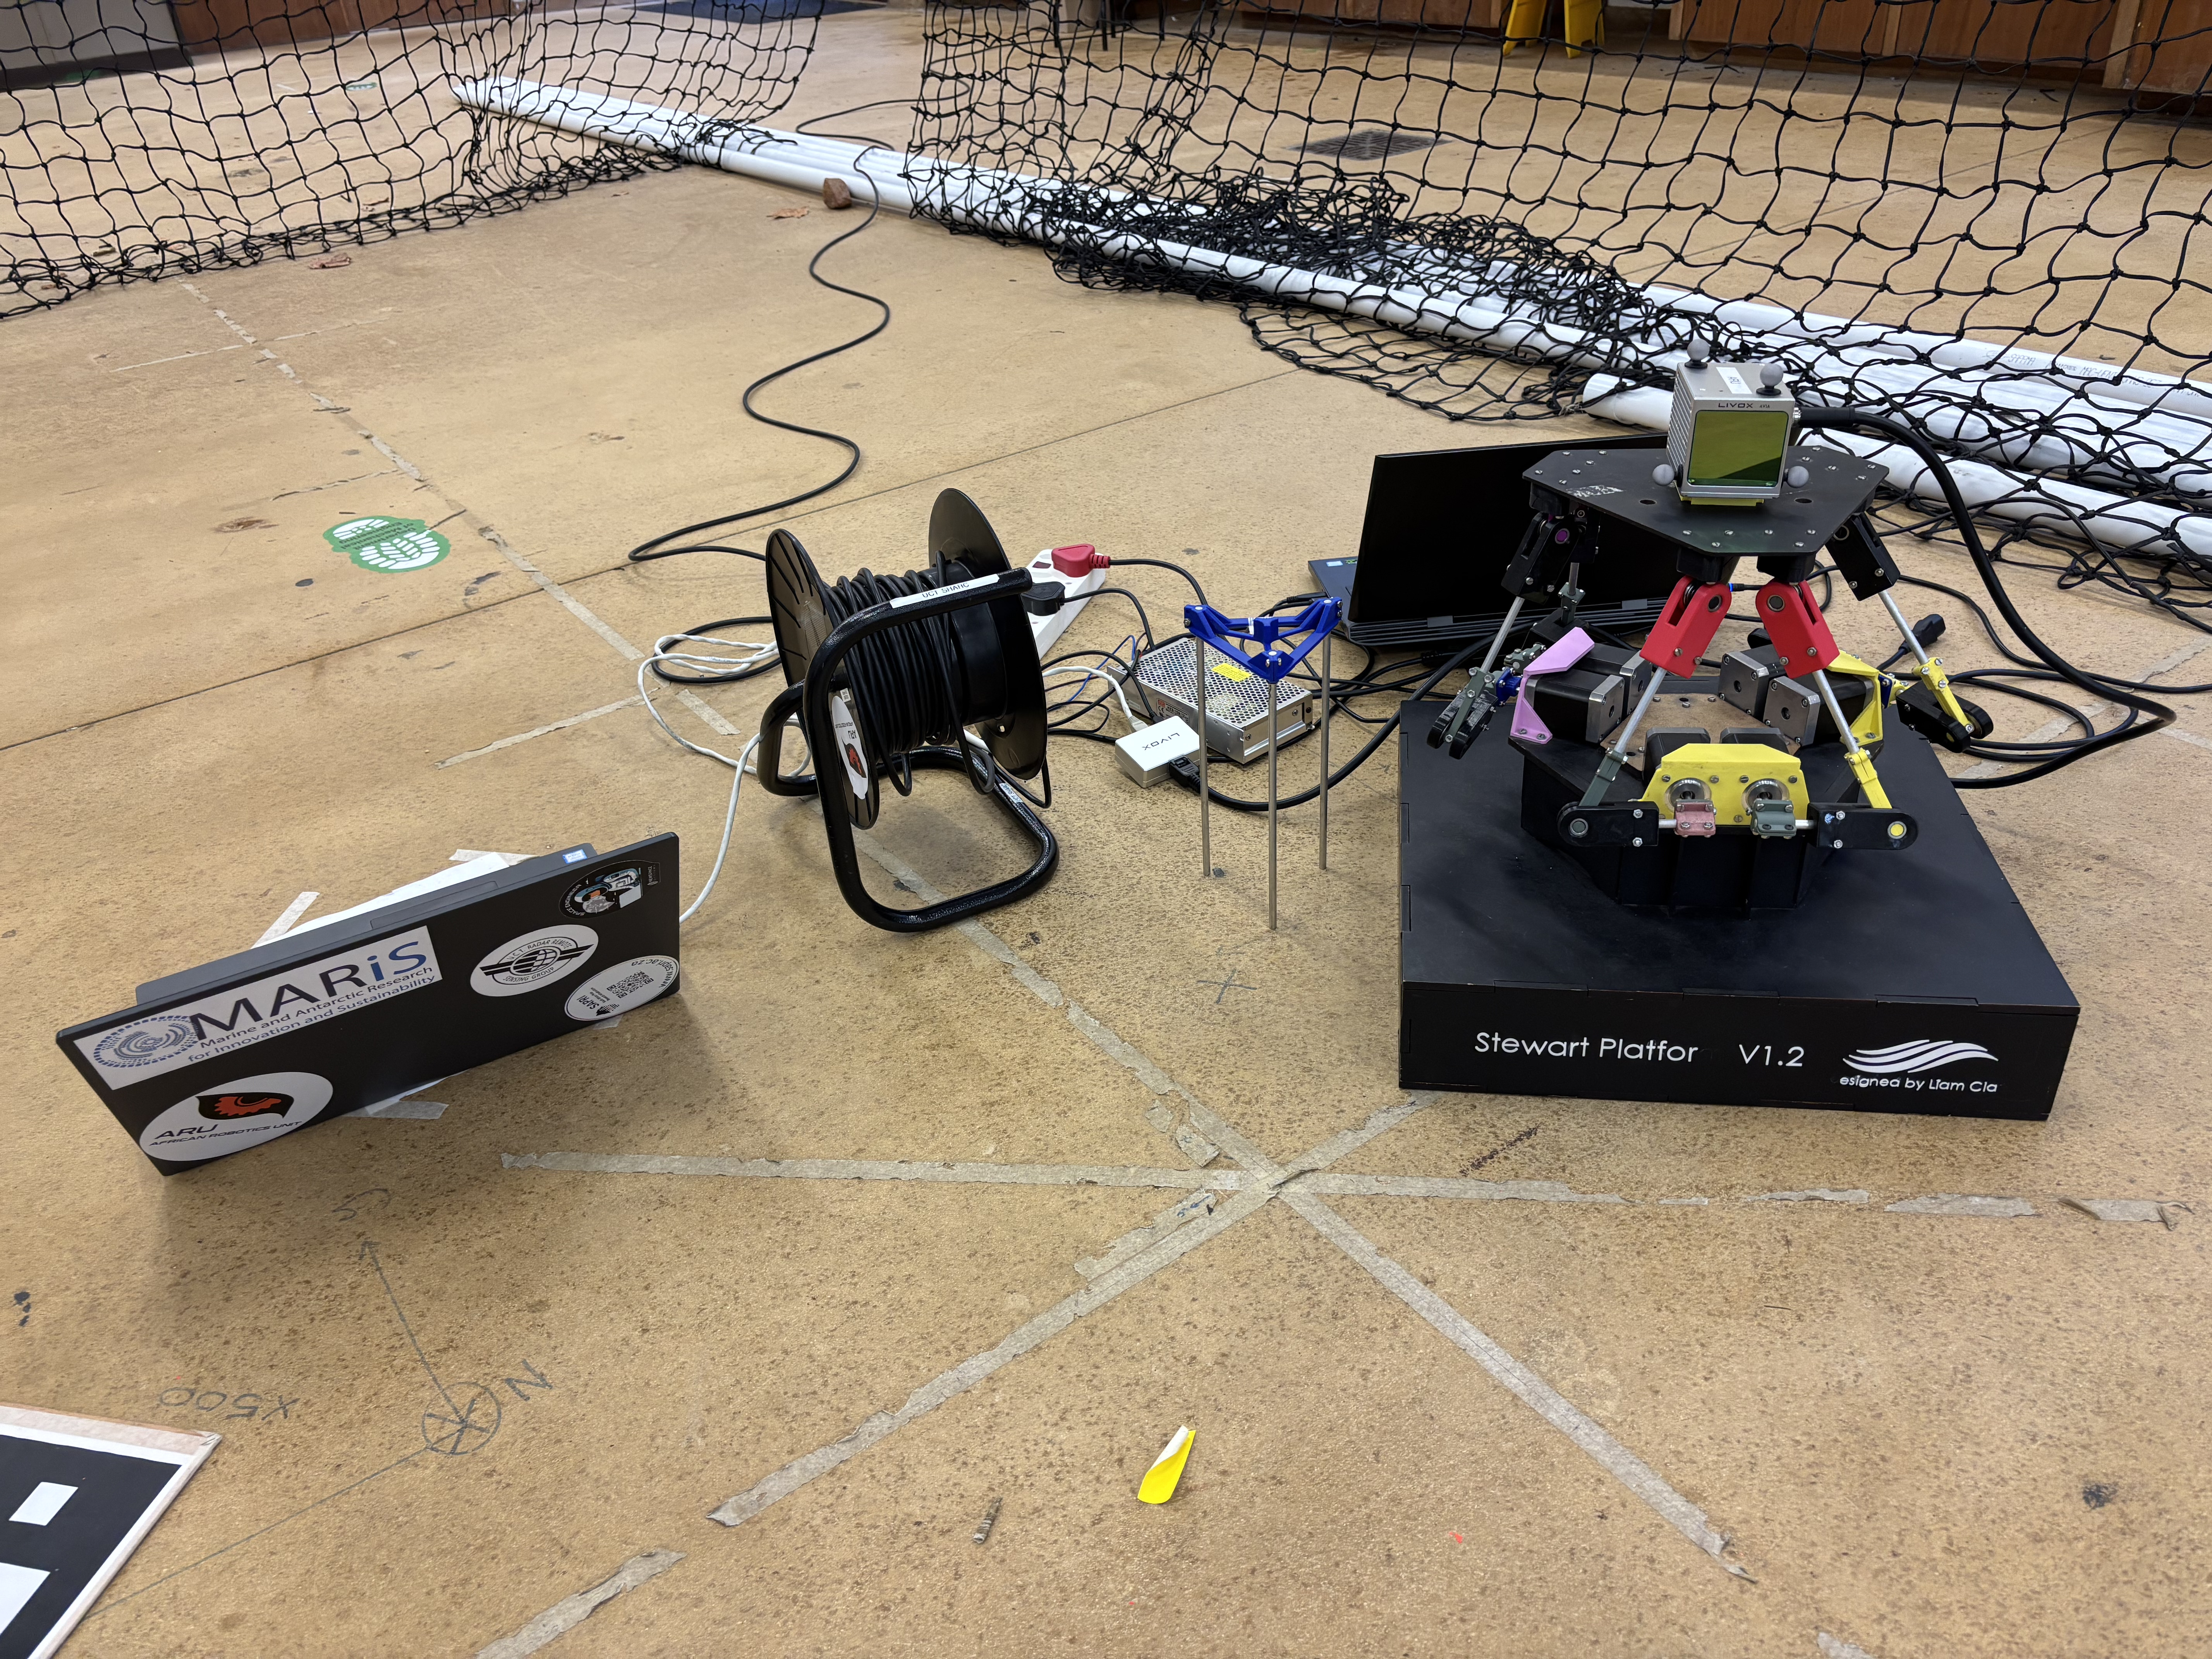
\includegraphics[width=0.95\linewidth]{figs/stewart_setup.jpg}
    %\caption{\textbf{Motion setup.}}
    %\label{fig:motion_setup}
  \end{minipage}%
  \begin{minipage}{.5\textwidth}
    \centering
    \includegraphics[width=0.95\linewidth]{figs/markers_1.png}
    %\caption{\textbf{Markers.}}
    %\label{fig:markers_1}
  \end{minipage}
  \caption{\textbf{Simulated Motion Experimental Setup.}}
  \label{fig:motion_setup}
\end{figure}
%----------------------------------------------------

%----------------------------------------------------
\begin{figure}[H]
\centering
\begin{minipage}{.5\textwidth}
    \centering
    \includegraphics[width=0.95\linewidth]{figs/markers_0.png}
    %\caption{\textbf{Markers.}}
    %\label{fig:markers_0}
  \end{minipage}%
  \begin{minipage}{.5\textwidth}
    \centering
    \includegraphics[width=0.95\linewidth]{figs/markers_2.png}
    %\caption{\textbf{Markers.}}
    %\label{fig:markers_2}
  \end{minipage}
  \caption{\textbf{Motion Capture Markers on Livox Avia.}}
  \label{fig:markers}
\end{figure}
%----------------------------------------------------

The Stewart platform was set to carry out two pre-defined motion routines of different amplitudes, while both the Avia's \ac{IMU} motion capture system recorded data. The routine consisted of:

\begin{enumerate}
    \item Rotation about the Avia's X-axis (roll)
    \item Rotation about the Avia's Y-axis (pitch)
    \item Rotation about both the Avia's X and Y-axes (roll and pitch)
    \item Rotation about the Avia's X, Y and Z-axes (roll, pitch and yaw)
\end{enumerate}

The frequency of each rotation was set to vary over time, following a chirp function, beginning at a frequency of 0.005 Hz and ending at a frequency of 0.05 Hz over a duration of 60 seconds. The first routine was carried out with a rotation amplitude of 10°, while the second routine was carried out with a rotation amplitude of 5°.

The amplitude and frequency parameters for the motion routines were selected to simulate the expected motion of a research vessel at sea. The \ac{IMU} data collected during the \ac{SCALE} Winter 2022 Cruise, detailed in Section \ref{subsec:ch4.section3.subsec2}, was inspected and informed the selection of these parameters. During the cruise, the Avia was mounted on the port side of the vessel several decks above the waterline, several meters from the stern. The vessel experienced moderate sea conditions during data collection, as no data was collected during poor weather. The resulting motion of the Avia during data collection was expected to be predominantly low amplitude and frequency pitch and roll motion, with a limited amount of yaw and translational motion.

\newpage
%====================================================
\section{Ice Field Data Collection}
\label{sec:ch4.section3}
%----------------------------------------------------

Two sets of ice field data, one simulated and one in-situ, were collected using the Livox Avia sensor. The simulated ice field data was collected at the Aalto University Ice and Wave Tank in Finland, while the in-situ ice field data was collected during the \ac{SCALE} Winter 2022 Cruise aboard the \textit{S.A. Agulhas II}. 

%----------------------------------------------------
\subsection{Aalto University Ice and Wave Tank}
\label{subsec:ch4.section3.subsec1}

Aalto University operates a wave and ice tank 40 m x 40 m and 2.8 m deep. The tank is equipped with 16 wedge-type plunger wave generators capable of producing regular and irregular waves (\cite{AaltoIceWave2024}). In addition to wave generators, the tank is equipped with a cooling system and sprayers for producing model-scale ice. The tank is used for a variety of research activities, including investigations into wave-ice interactions, ice mechanics, and coastal engineering.

%----------------------------------------------------
\begin{figure}[H]
    \centering
    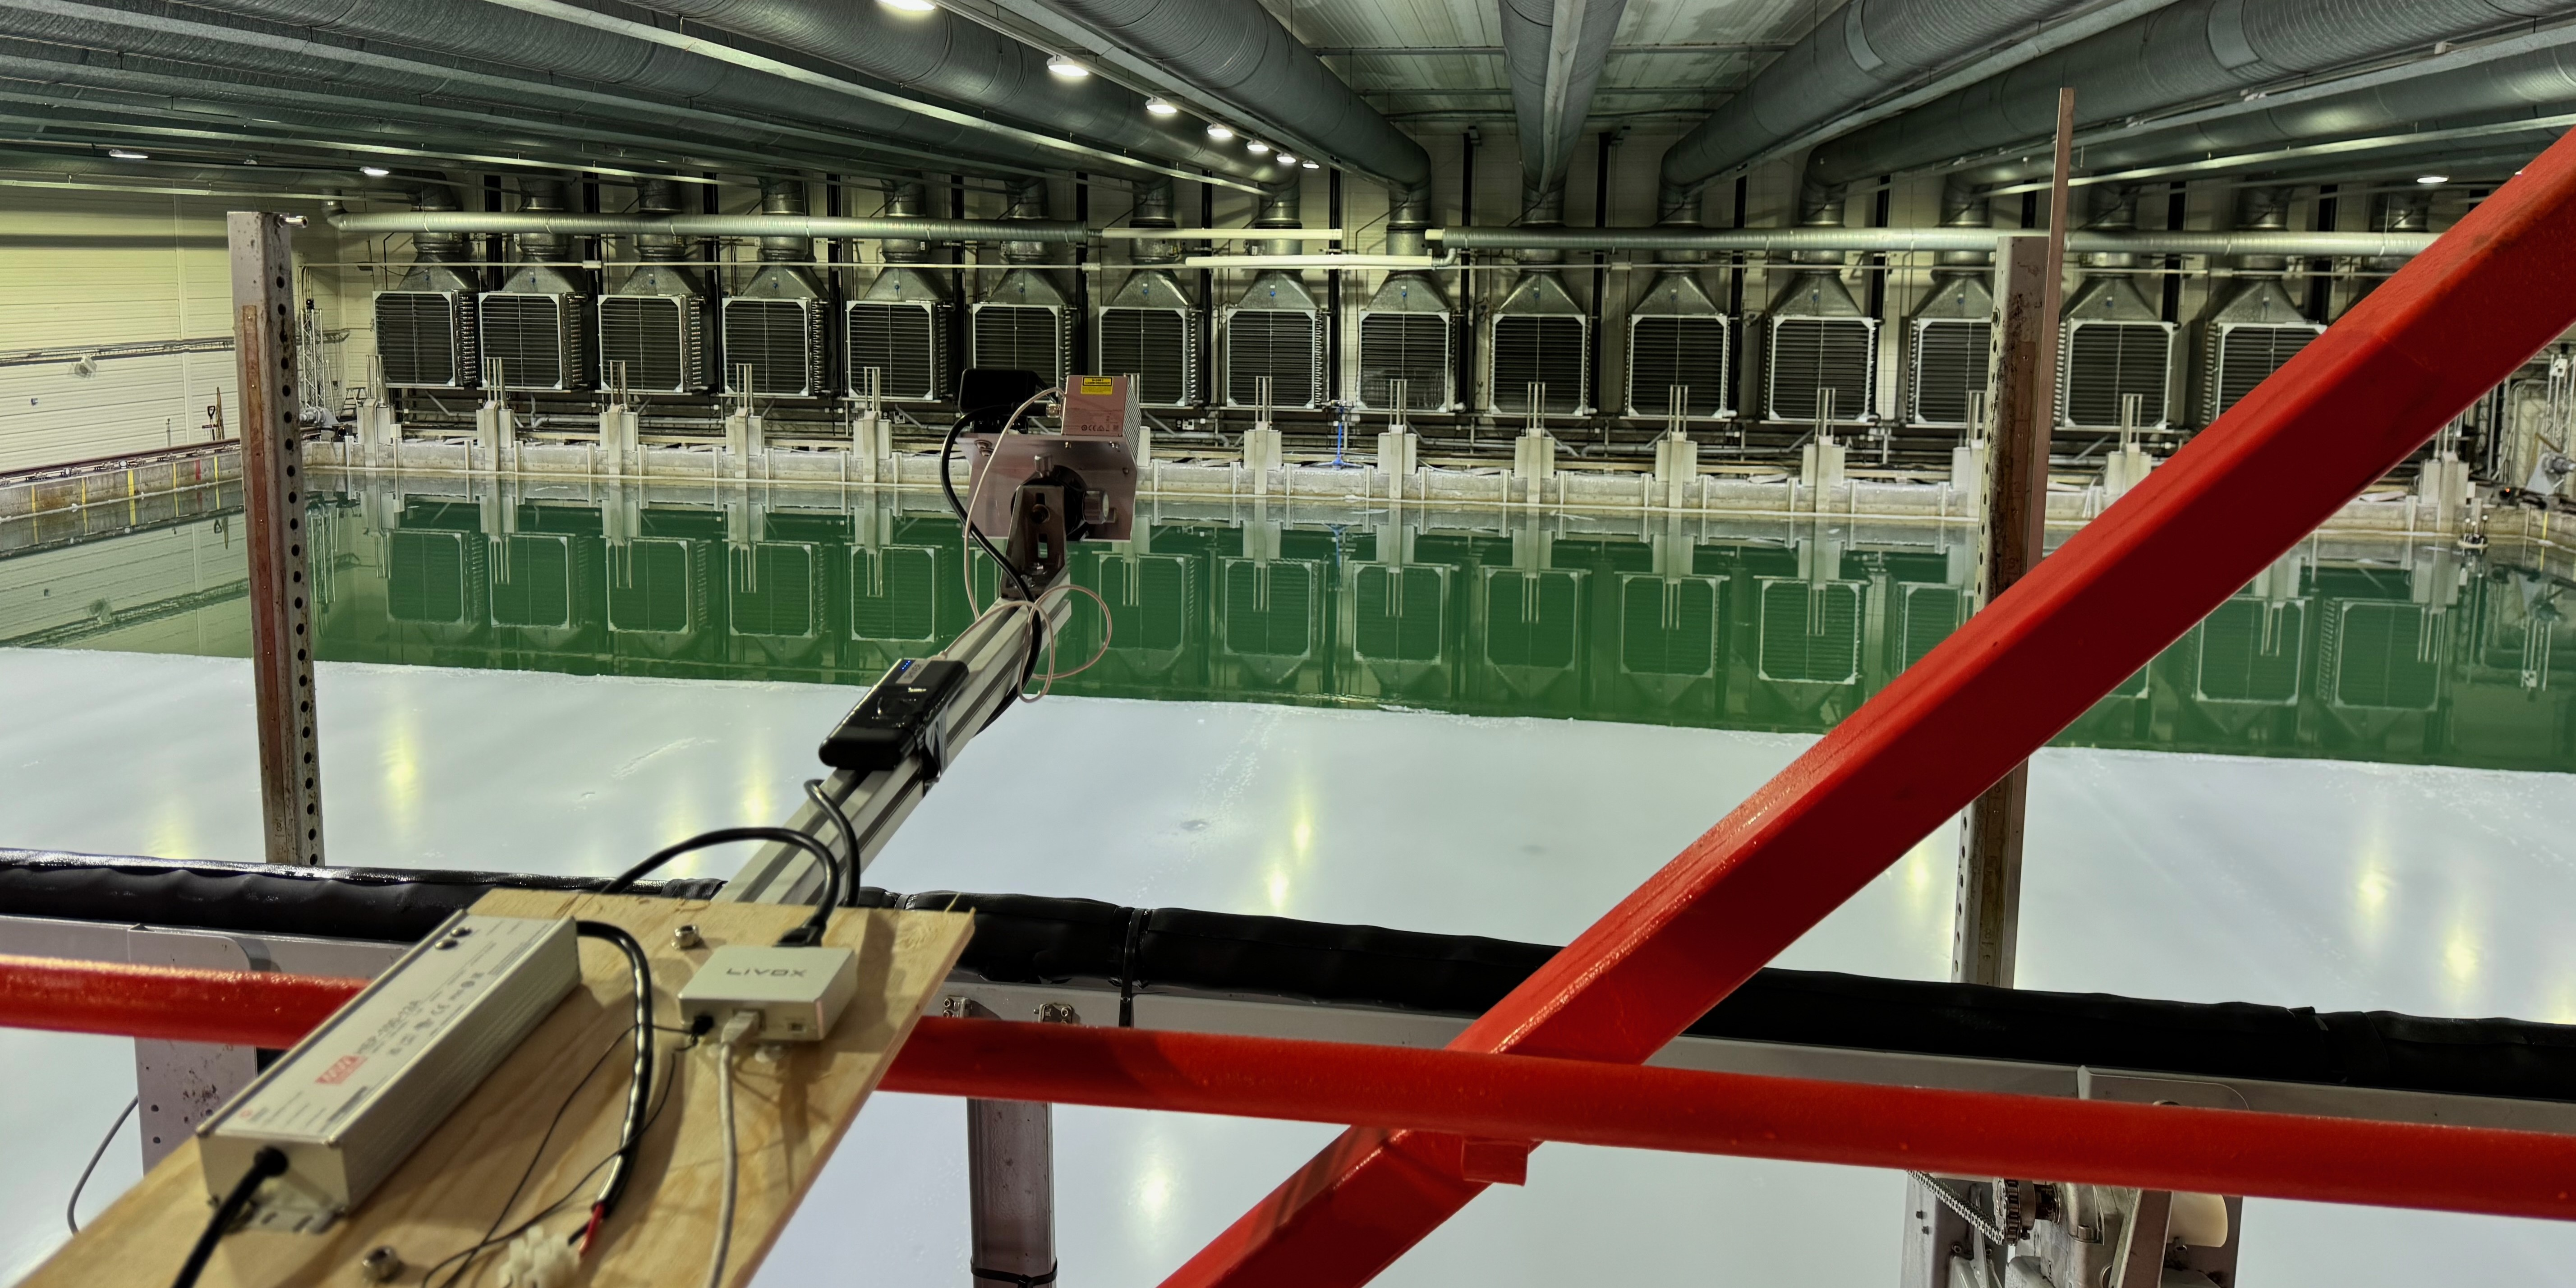
\includegraphics[width=0.9\textwidth]{figs/Aalto_Livox.jpeg}
    \caption{\textbf{Livox Avia at Aalto University Ice and Wave Tank.} R.A. Verrinder.}
    \label{fig:aalto}
\end{figure}
%----------------------------------------------------

In November 2023, a fellow Masters student (\cite{nairThreeDimensionalComputational2024}) ran experiments in the tank to simulate the motion of an individual pancake ice floe using a scale model. In addition to the sensors selected by Nair for his experiments, point cloud data from these tests were collected using the Avia.
The Avia was mounted on a mobile gantry above the tank, angled to face down towards the ice and water, in the direction of the wave generators. Waves were generated and briefly propagated through open water before reaching the ice.  A capacitive probe in the tank recorded the wave height over time, and was placed 5 meters in front of the wave generators. The wave data was sampled at a rate of 300 Hz.

A uniform sheet of ice was created in the tank before the tests (any idea of ice thickness?). Throughout the experiment, the ice sheet progressively broke up into individual ice floes due to the generated wave action. No addition ice was created during the experiment.

Six individual tests were carried out during the experiment, with varying wave heights and periods. For all tests, sinusoidal waves were generated at two periods, with three wave heights per period, see Table \ref{tab:tank_tests}. During these tests there was no time synchronisation between the wave probe logging and Livox Avia.

%----------------------------------------------------
\begin{table}[H]
\centering
\caption{Wave Tank Test Parameters.}
\begin{tabular}{|l|r|r|}
\hline
\textbf{Test} & \multicolumn{1}{l|}{\textbf{Amplitude (mm)}} & \multicolumn{1}{l|}{\textbf{Period (s)}} \\ \hline
1 & 25   & 1.6 \\ \hline
2 & 37.5 & 1.6 \\ \hline
3 & 50   & 1.6 \\ \hline
4 & 25   & 2   \\ \hline
5 & 37.5 & 2   \\ \hline
6 & 50   & 2   \\ \hline
\end{tabular}
\label{tab:tank_tests}
\end{table}
%----------------------------------------------------

During the tests, strict constraints were placed on the waves generated and their behaviours. The generated waves were all sine waves in deep water (the water depth is greater than half the largest generated wavelength, 2.8 m $>$ 2 m). The wave parameters were held constant during individual tests, and the waves were propagated straight down the tank, towards the Avia. 

%----------------------------------------------------
\subsection{SCALE Winter 2022 Cruise}
\label{subsec:ch4.section3.subsec2}

The \ac{SCALE} Winter 2022 Cruise was a research cruise aboard then Research Vessel \textit{S.A. Agulhas II} that took place from the 11th to the 31st of July 2022. Amongst other data collection and research activities taking place on the vessel, 31 \ac{LiDAR} scans of the open ocean and ice fields in the \ac{MIZ} were taken, between the 15th and the 27th of July. Of these 31 scans, 12 were of scenes containing ice fields or pancake ice floes. The remaining 19 scans were either setup scans or of scenes of open water without ice. All scans of ice were taken between 58° and 59°35' South.

%----------------------------------------------------
\begin{figure}[H]
    \centering
    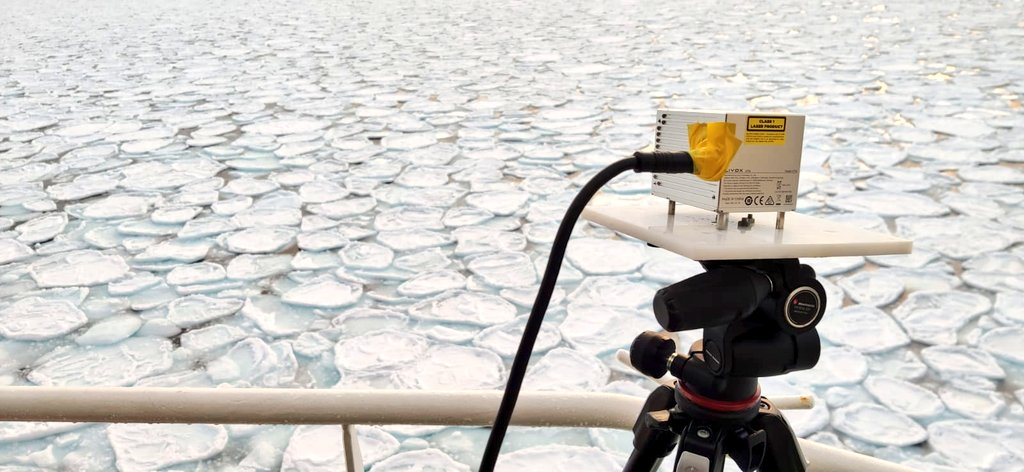
\includegraphics[width=0.9\textwidth]{figs/lidar.jpg}
    \caption{\textbf{Livox Avia above Pancake Ice.} A. Spirakis.}
    \label{fig:lidar}
\end{figure}
%----------------------------------------------------

Data were collected from the port side 7th floor deck, at a height of approximately 16-17 m above the waterline, with the sensor angled downwards towards the ocean at an angle of approximately 20° from the horizontal, see Figure \ref{fig:setup}. A video camera was mounted several decks above the Avia, facing down towards the ocean, captured video footage continuously throughout the voyage. Although the camera was primarily used for a separate research activity and did not have the same \ac{FOV} as the Avia, the footage provided useful visual context for the \ac{LiDAR} data collected.

%----------------------------------------------------
\begin{figure}[H]
    \centering
    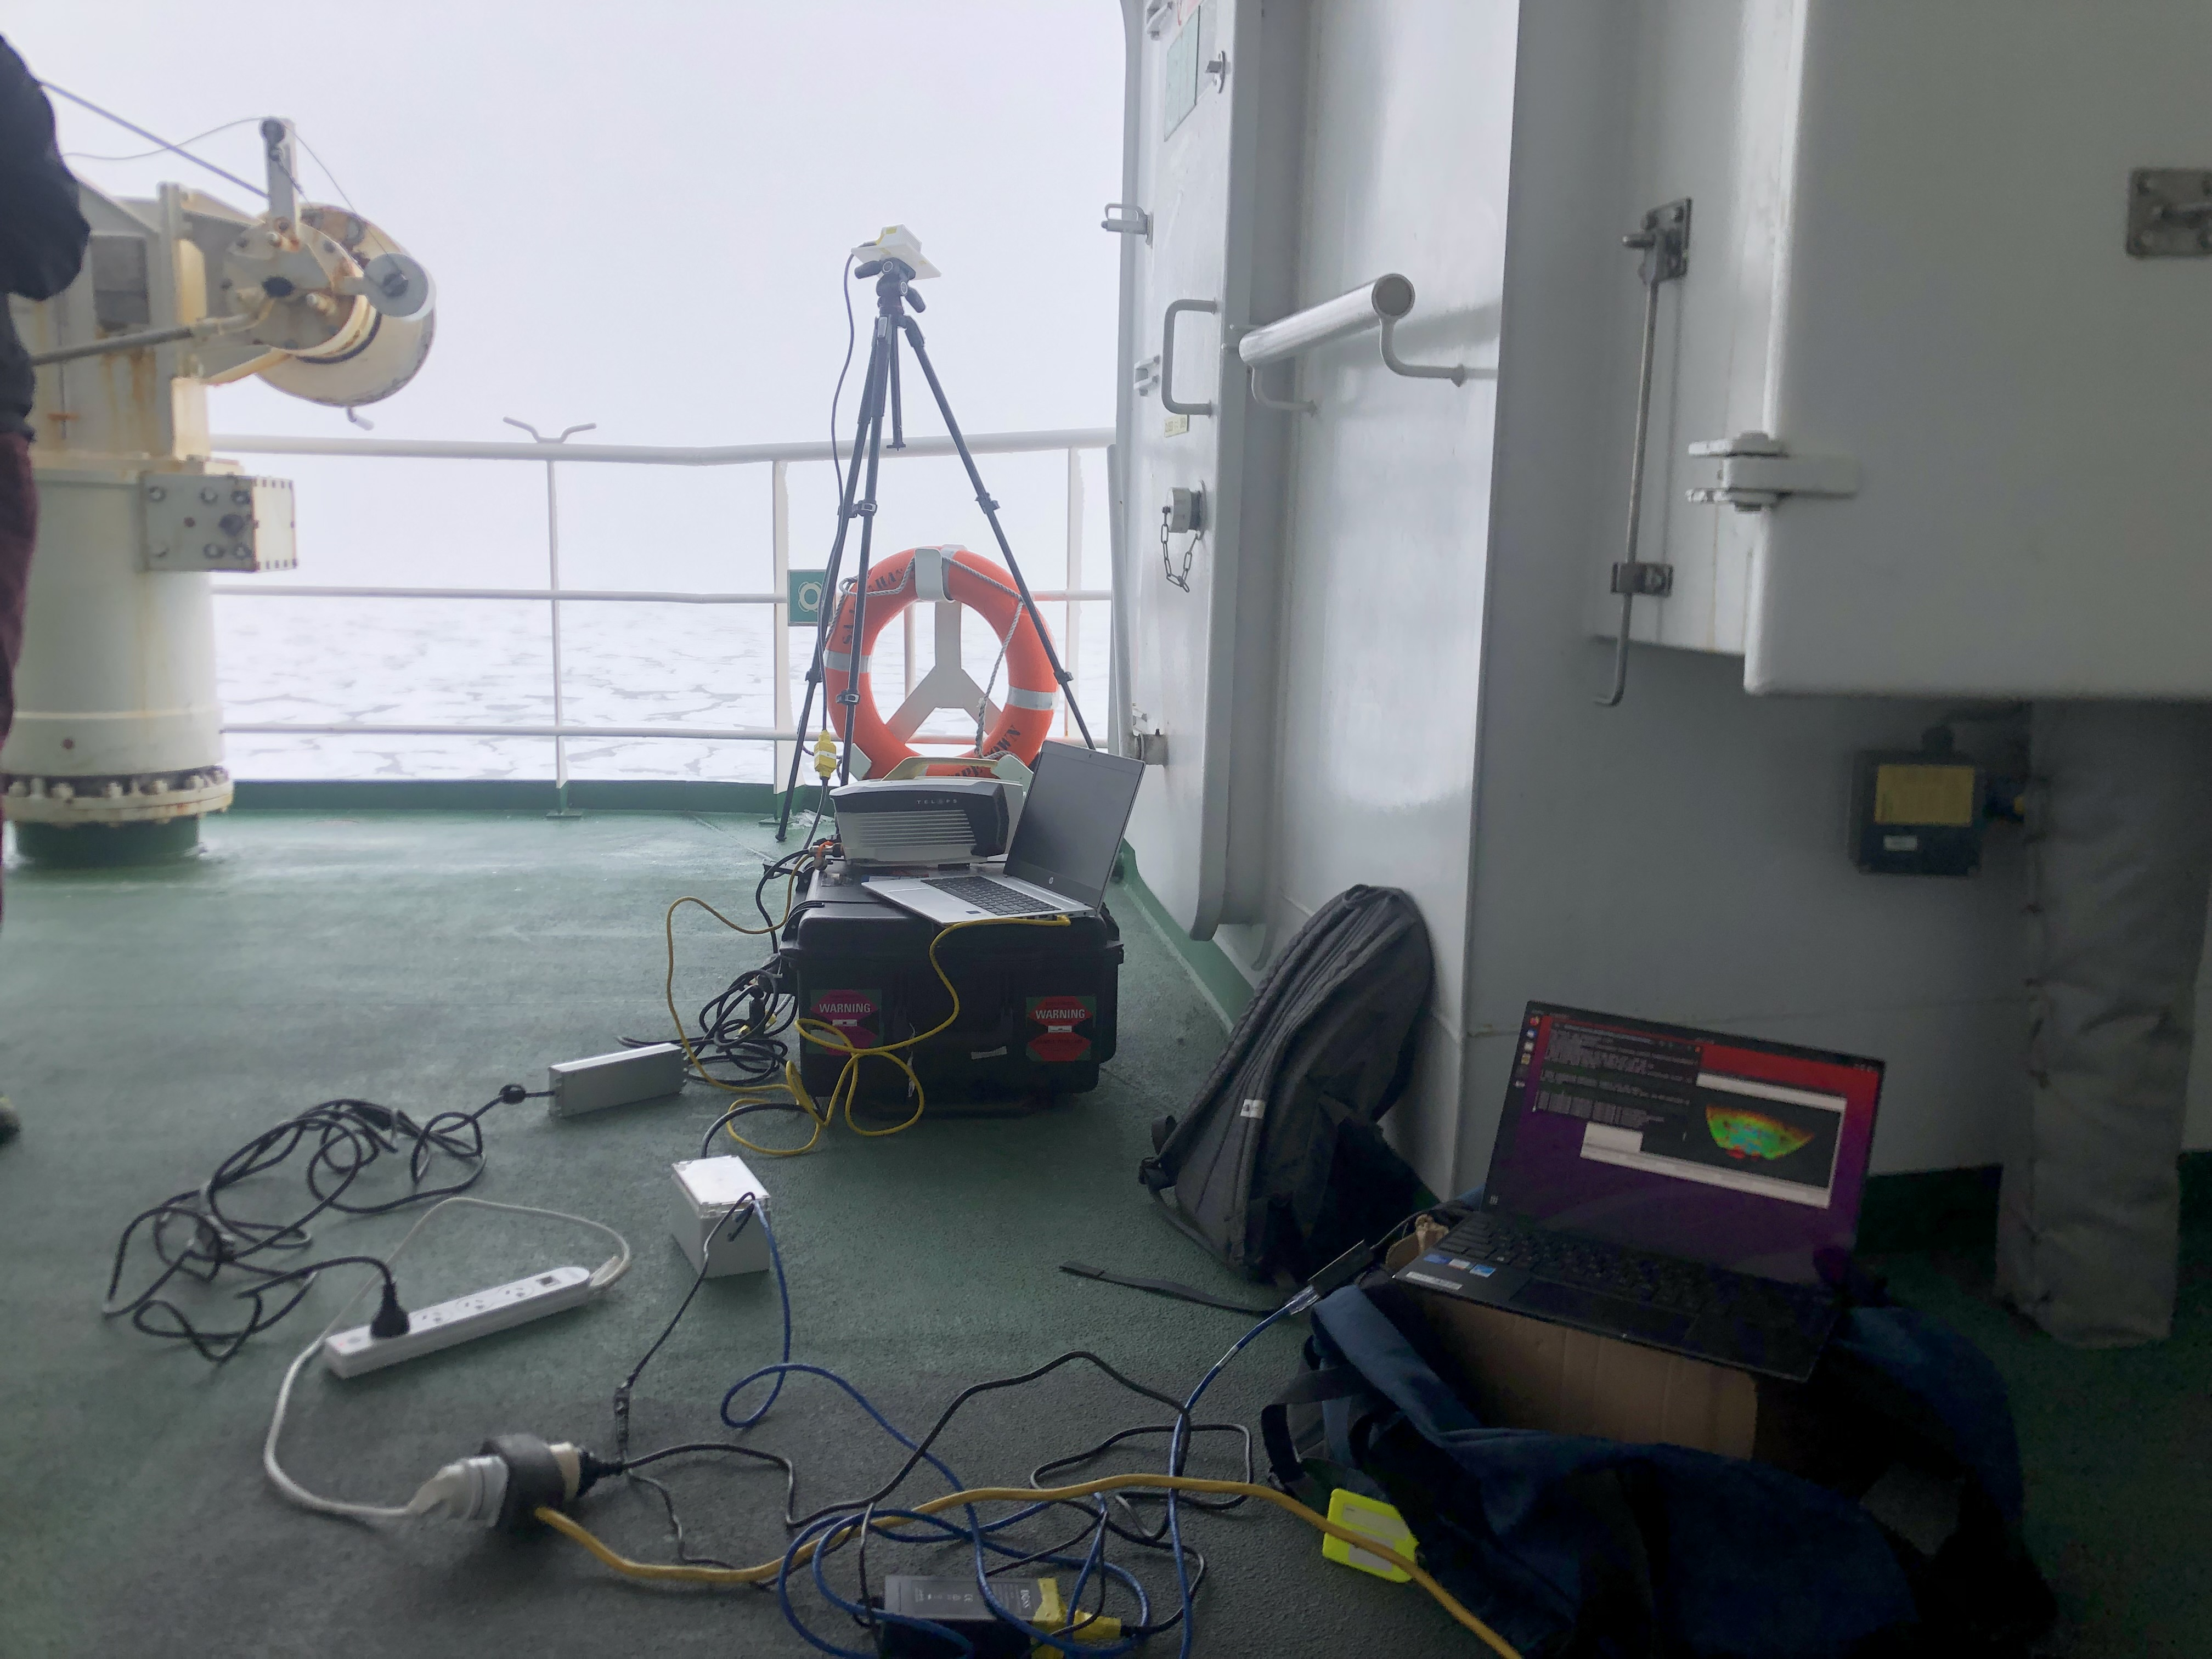
\includegraphics[width=0.9\textwidth]{figs/setup.jpg}
    \caption{\textbf{Data Collection Setup.} A. Spirakis.}
    \label{fig:setup}
\end{figure}
%----------------------------------------------------

*insert map here?*

%----------------------------------------------------
\begin{figure}[H]
    \centering
    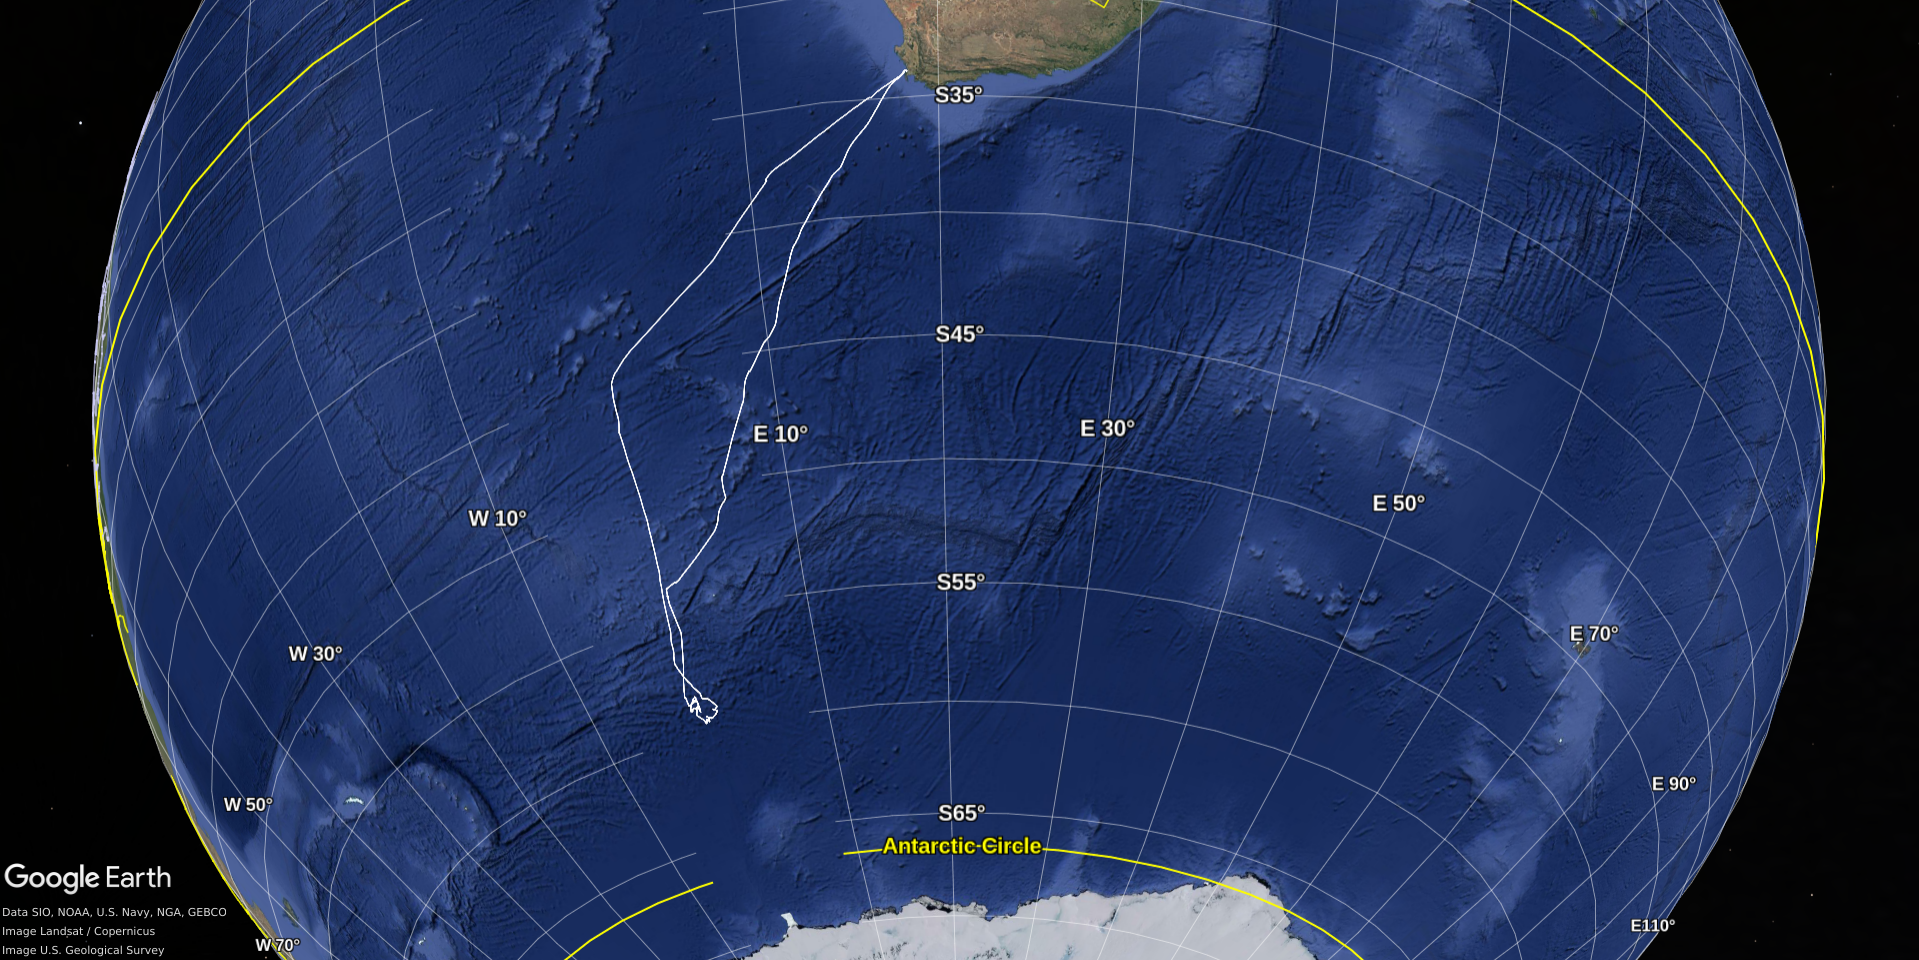
\includegraphics[width=0.9\textwidth]{figs/map.png}
    \caption{\textbf{SCALE Winter 2022 Cruise Track.}}
    \label{fig:map}
\end{figure}
%----------------------------------------------------

%****************************************************
% END
%****************************************************